%%%%%%%%%%%%%%%%%%%%%%%%%%%%%%%%%%%%%%%%%%%%%%%%%%%%%%%%%%%%%%%
\section{Jets}\label{sec:jets}
%%%%%%%%%%%%%%%%%%%%%%%%%%%%%%%%%%%%%%%%%%%%%%%%%%%%%%%%%%%%%%%

Particles carrying a color charge, such as quarks, cannot exist in free form because of QCD confinement which only allows for colorless states (\FIXME{point here to theory chapter}). Quarks and gluons interact with pairs of quarks and anti-quarks produced from the vacuum until the formation of stable colourless hadrons, the process is called hadronization. The ensemble of the final colourless objects is called a jet and it is reconstructed in the detector from energy depositions and charged particle momenta.
The jets point back to the primary interaction, i.e. to the partons the jets originated from, but a correction for hadronization and detector effects is needed. Jet clustering algorithms have been developed to cluster particles (at parton, particle or detector level) into jets and reconstruct the energy and direction of the original parton. The task of a jet clustering algorithm is to allow comparisons between theoretical predictions, which are usually described by perturbative calculations, and experimental data. This is achieved reducing the complex structure of particle jets from a scattered parton to a simple four-momentum, which represents the main property of particle jets.
In order to guarantee a meaningful calculation of theory predictions, jet clustering algorithms are characterized by two important properties.
%Two properties of jet clustering algorithms are desired to be able to calculate meaningful theory predictions.
Clustering algorithms need to be infrared-safe, which means that the emission of infinitesimally-low-energy partons from partons inside a jet does not affect the jet properties. Furthermore, they need to be collinear-safe, which means that jet properties are not affected by the splitting of a parton inside a jet into two collinear partons.
Jet algorithms for hadron colliders can be divided into two classes: cone~\cite{Salam:2007xv} and sequential clustering~\cite{Catani:1993hr,Ellis:1993tq,Dokshitzer:1997in,Wobisch:1998wt,Cacciari:2008gp} algorithms.
%Jet algorithms for hadron colliders can be divided into two classes. One possibility is based on proximity in coordinate space, cone jet algorithms [180, 181]) whereas the other uses proximity in momentum space by successively merging pairs of particles in order of increasing relative transverse momentum, kT algorithms [182, 183]). For this work only the anti-kT algorithm of the kT family is used and detailed in the following.
The main algorithms used by LHC experiments are the anti-$k_t$ algorithm~\cite{Cacciari:2008gp} (AK) and the Cambridge--Aachen (CA)~\cite{Catani:1993hr,Dokshitzer:1997in} algorithms, which are found to fulfil theory requirements and to exhibit good properties for experimental measurements. For this work both algorithms are used and described in the following.
 
 %%%%%%%% 
\subsection{Jet clustering algorithms}\label{subsec:jetsalgo}
%%%%%%%%

In sequential jet clustering algorithms, jets are defined through sequential, iterative procedures that combine four-vectors of input pairs of particles until certain criteria are satisfied and jets are formed. In particular, for each pair of particles $i$ and $j$, a distance variable between the two particles ($d_{ij}$), and the so-called ``beam distance'' for each particle ($d_{iB}$), are computed:
 
\begin{equation}
d_{ij} = \mathrm{min}(p_{Ti}^{2n},p_{Tj}^{2n})\frac{\Delta R^2{ij}}{R^2}\quad,\quad\quad\quad
d_{iB} = p_{Ti}^{2n}\quad,
\end{equation} 

where $p_{Ti}$ and $p_{Tj}$ are the transverse momenta of particles $i$ and $j$, respectively, ``min'' refers to the smaller of the two \pt values, the integer $n$ depends on the specific jet algorithm, $\Delta R^2{ij}$ is the distance between $i$ and $j$ in $\eta$ and $\phi$, and $R$ is a free distance parameter, with all angles expressed in radians. The particle pair ($i$, $j$) with smallest $d_{ij}$ is combined into a single object. All distances are recalculated using the new object, and the procedure is repeated until, for a given object $i$, all the $d_{ij}$ are greater than $d_{iB}$. Object $i$ is then classified as a jet and not considered further in the algorithm. The process is repeated until all input particles are clustered into jets.

The distance parameter $R$ is responsible for defining the angular size of the jet. The parameter $n$ governs the topological properties of the jets and depending on its value three different classes of clustering algorithms are distinguished. For $n = 1$ the procedure is referred to as the $k_t$ algorithm (KT), which clusters soft objects before harder ones are added to the final jet. The KT jets tend to have irregular shapes and are especially useful for reconstructing jets of lower momentum~\cite{Cacciari:2008gp}. For this reason, they are also sensitive to the presence of low-\pt pileup contributions.
%, and are used to compute the mean \pt per unit area of an event.
For $n = 0$, the procedure corresponds to the CA algorithm. This relies only on angular information, and, like the KT algorithm, provides irregularly-shaped jets. The CA algorithm is useful in identifying jet substructure as described in Chapter~\ref{ch:vtagging}. For $n = -1$, the procedure corresponds to the AK algorithm, which compares the inverse square of the transverse momenta.
The AK algorithm is used extensively in LHC experiments and by the theoretical community for finding well-separated jets. The use of inverse square of the \pt as a weight in the $d_{ij}$ distances has the advantage that hard objects collect adjacent soft ones before these are clustered among themselves into harder objects, figuratively reproducing in reverse the parton fragmentation and gluon emission processes.
This property makes the algorithm independent on soft radiation preserving infrared-safety. The AK algorithm is also collinear-safe as the clustering is driven by the angular distance between two particles. Gluons emitted at small angles are picked up by the algorithm in early steps of the iteration and therefore do not affect the jet properties. Furthermore, this algorithm tends, by construction, to form almost circular jets allowing for straight-forward calibration and understanding of the detector acceptance. The behaviours of the CA and AK jet algorithms are illustrated in Fig,~\ref{fig:jetalgos}. 
%This algorithm is collinear-safe as the clustering is driven by the angular distance between two particles. Gluons emitted at small angles are picked up by the algorithm in early steps of the iteration and therefore do not affect the jet properties. The algorithm is also infrared-safe. Due to the weighting with the inverse maximum squared transverse momentum, the emission of additional low energy gluons are picked up rather late in the clustering process. They are picked up after all hard emissions at small angles, but, importantly, before two soft particles can cluster with each other. Soft emissions will therefore not cluster into separate jets, preserving infrared-safety.
%The AK algorithm has very good experimental properties. By construction it tends to form almost circular jets with a radius of R. This is demonstrated for an example event in Fig. 7.1. Only if two jets are closer than 2R, the shape of the two jets varies from being circular. Experimentally this feature is very important as it allows straight-forward calibration and un- derstanding of the detector acceptance. Due to its limited cone size, the measurement of jets can be restricted to active detector regions. Due to the fixed cone size, the number of detector cells to be clustered into a jet is constant over certain detector regions and therefore straight-forward to calibrate.

\begin{figure}[!htb]
\centering
\subfigure[]{\label{fig:jetalgos_a}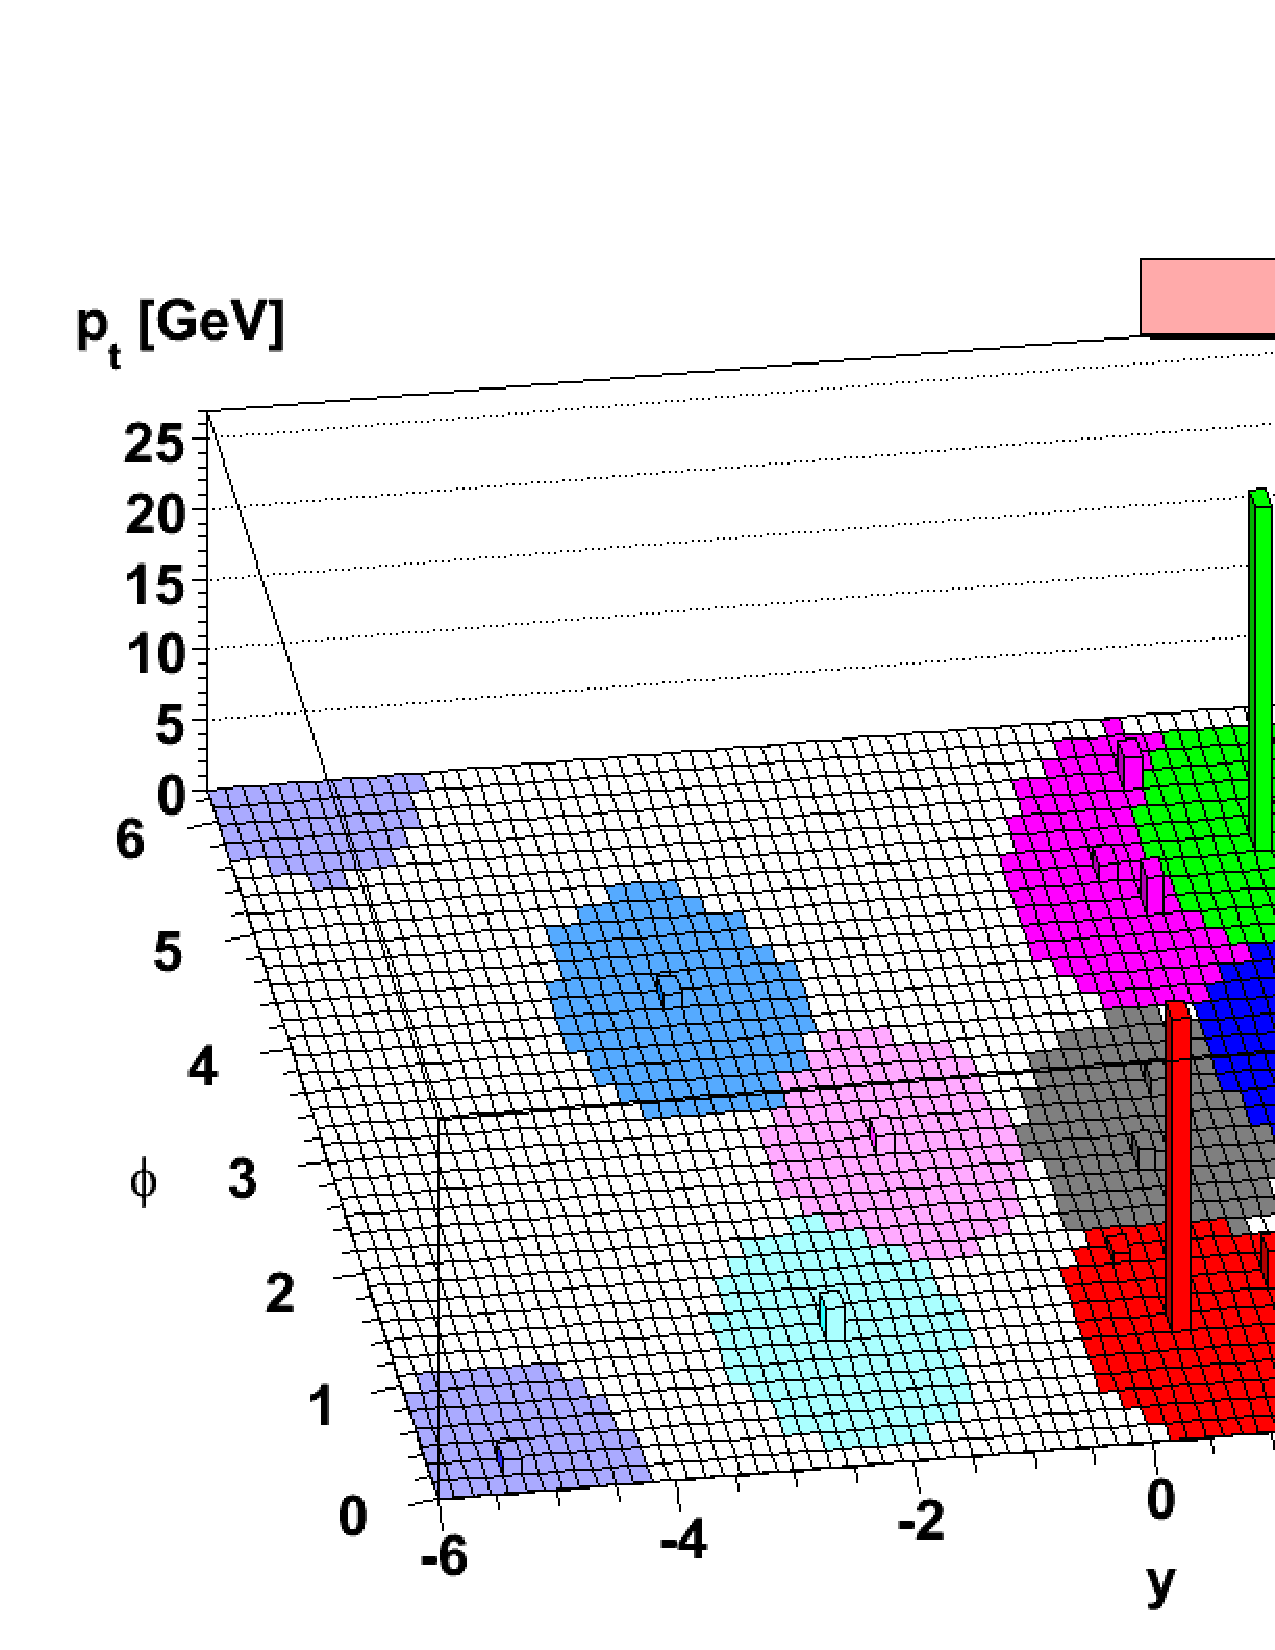
\includegraphics[width=0.4\textwidth]{\chsix/herwig-parton-level-ev-antikt-R1p0-ghosted4root.pdf}}
\subfigure[]{\label{fig:jetalgos_b}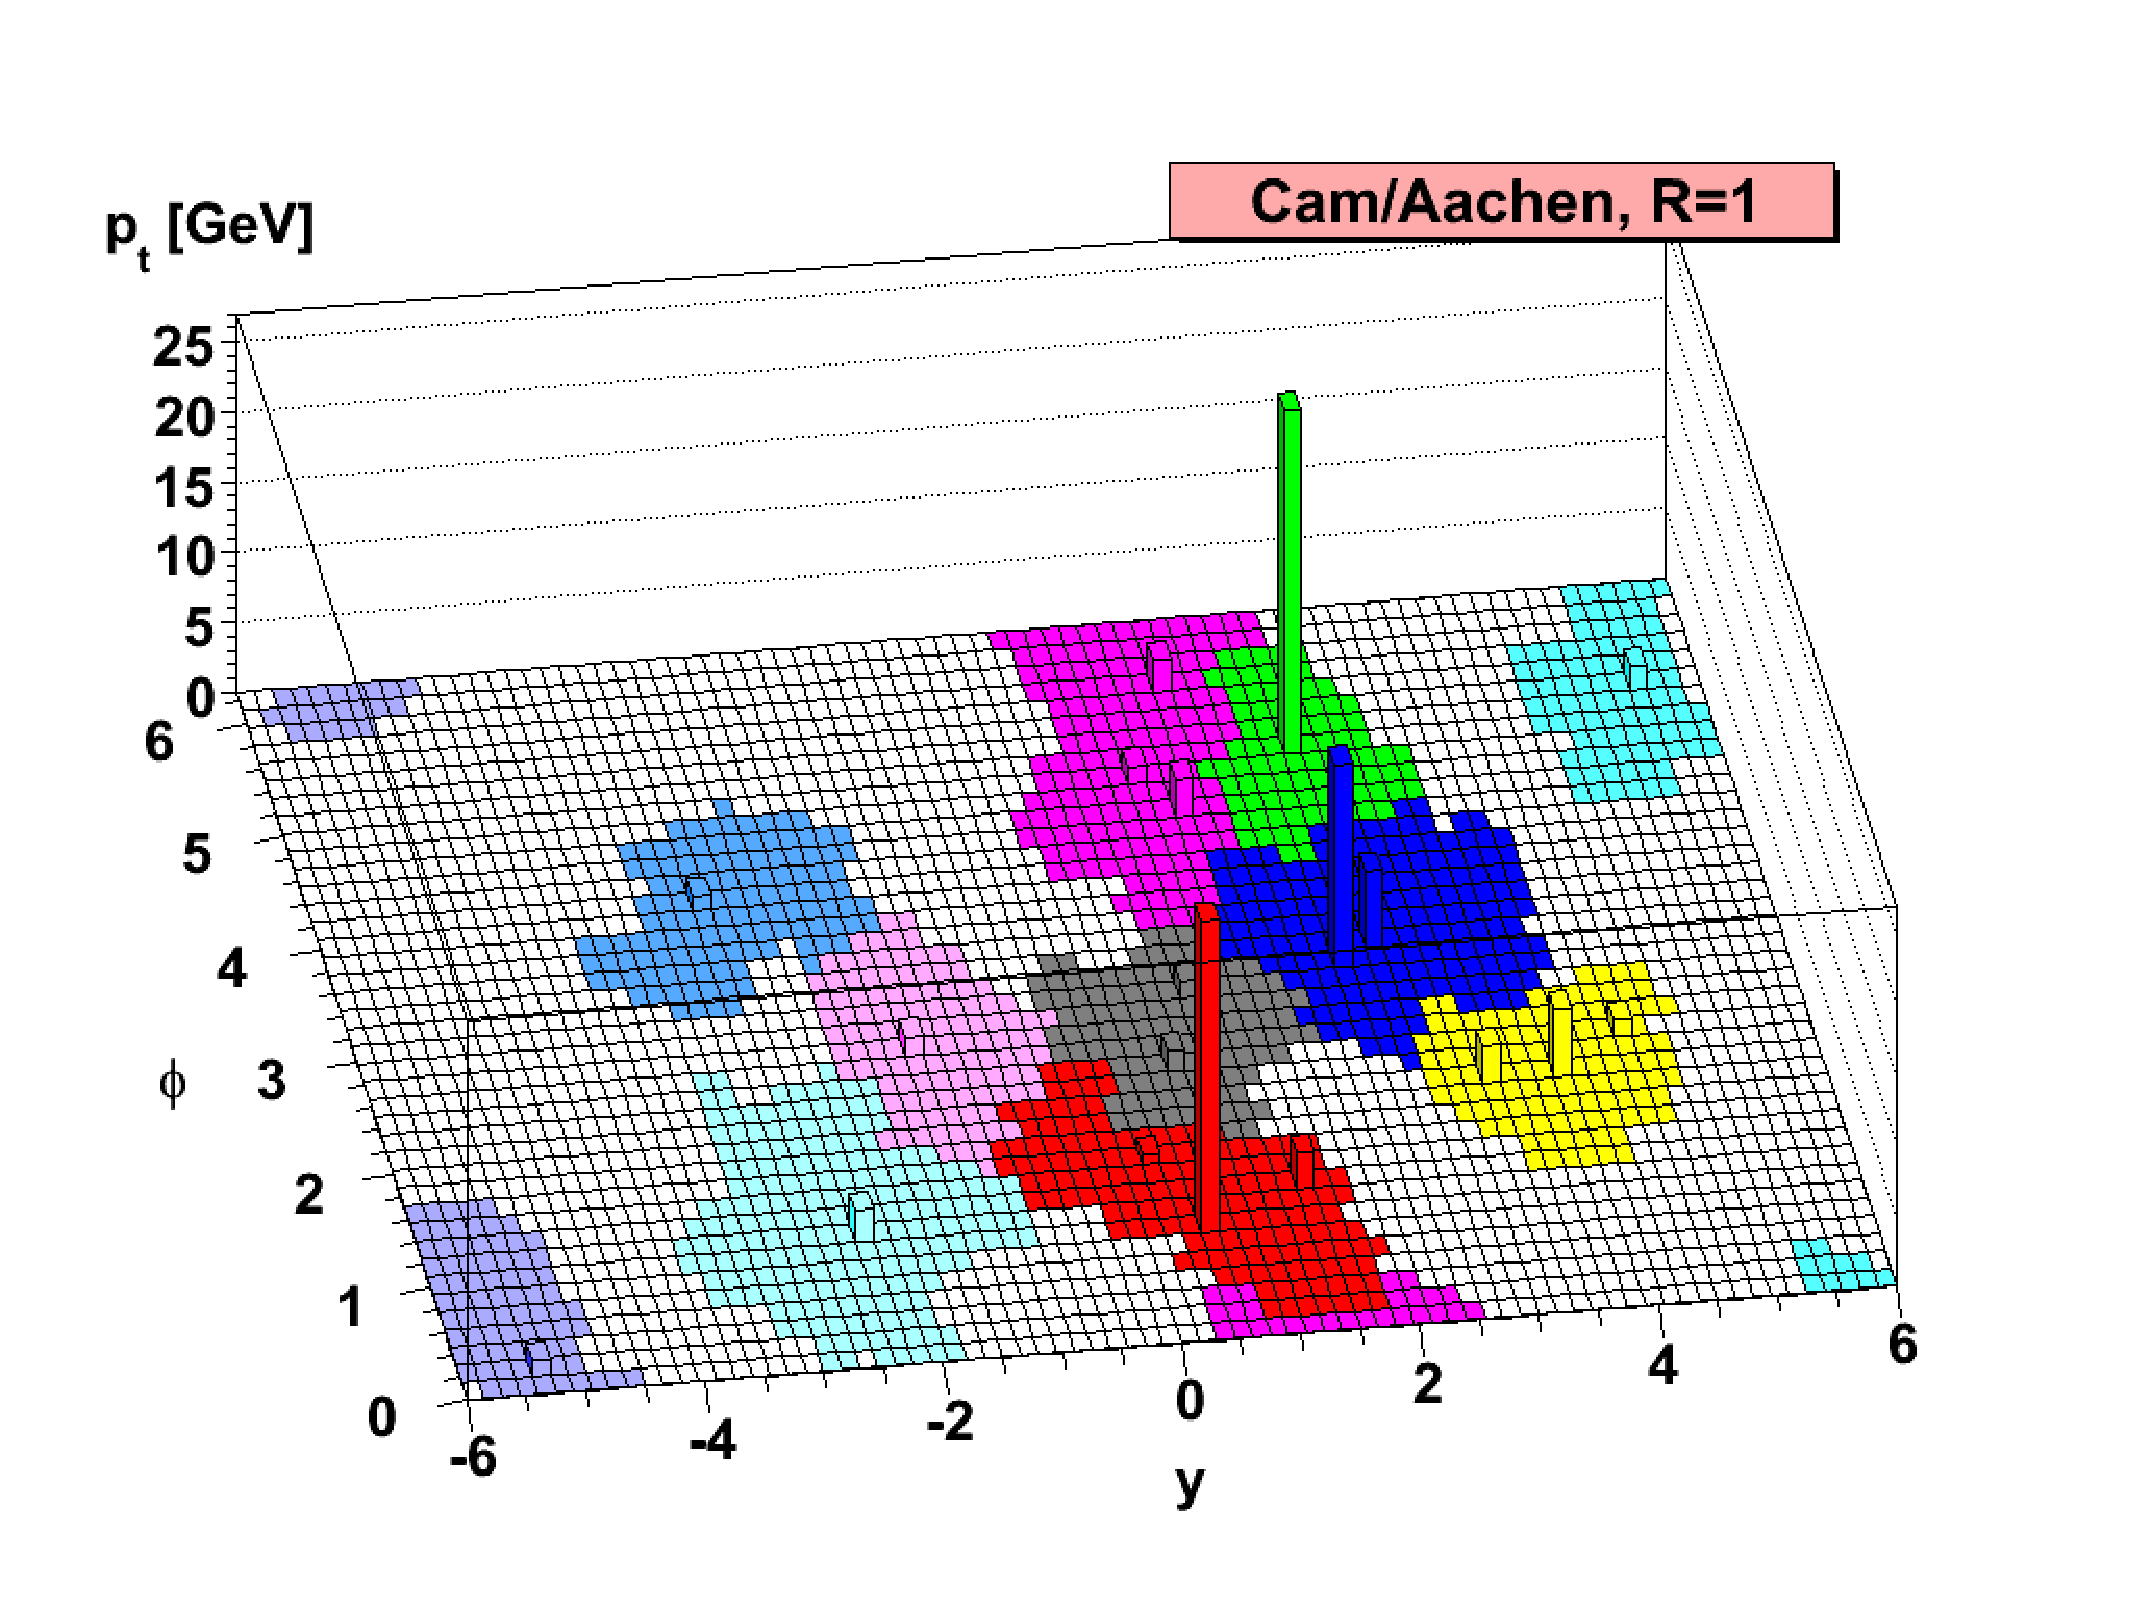
\includegraphics[width=0.4\textwidth]{\chsix/herwig-parton-level-ev-cam-R1p0-ghosted4root.pdf}}
\caption{An example of jet clustering with the AK (a) and CA (b) algorithms. The reconstructed jets are shown as colored regions~\cite{Cacciari:2008gp}.}
\label{fig:jetalgos}
\end{figure}

The choice of the distance parameters $R$, generally depends on the analysis. While large cone size jets collect all energy from the scattered parton, they also pick up a large contribution of background energy from the underlying event or pileup interactions. Small cone size jets pick up little contamination, but may not collect all energy from the scattered parton. 
The default choice in CMS for physics analyses at 8 and 13 TeV uses the KT algorithm with $R$ = 0.5 (AK5) and $R$ = 0.4 (AK4), respectively, since more collimated jets are expected at higher $\sqrt{s}$.
However, a larger value of $R$ increases the efficiency to entirely reconstruct the highly energetic products from boosted V$\rightarrow\qqbarpr$ and H$\rightarrow\bbbar$ decays. In fact, the average angular distance between the decay products is inversely proportional to the \pt of the mother particle. The default choice in CMS for physics analyses involving boosted V or H bosons decaying hadronically is $R = 0.8$. In particular, CA8 and AK8 jets are used in the 8 and 13\TeV analyses, respectively. The chosen value of $R$ provides a high efficiency for V or H bosons with small boost and ensures that no efficiency is lost in the transition from classical V/H reconstruction in two small jets at low V/H \pt and reconstruction from a single `large-cone jet at higher V/H \pt. Another point to consider when choosing the value of $R$, is the \ttbar data sample available for validating highly boosted V/H jets (see Section~\ref{sec:vtagging}). If $R$ is chosen too large, the b quark from the t$\rightarrow$Wb decay tends to merge into the W jet. The chosen value of $R$ is the result of a compromise between high efficiency for V/H bosons with small boost and a sufficiently large sample of W jets in \ttbar data for validating the V/H jet identification algorithms. Figure~\ref{fig:ca8effVsPt} shows the \pt range of W bosons for which the CA8 algorithm is efficient and compares this to the efficiency for reconstructing W bosons from two AK5 jets. Above a \pt of 200\GeV, the CA8 jet algorithm, used to identify W jets, becomes more efficient than the reconstruction of a W boson from two AK5 jets.

\begin{figure}[!htb]
 \begin{center}
  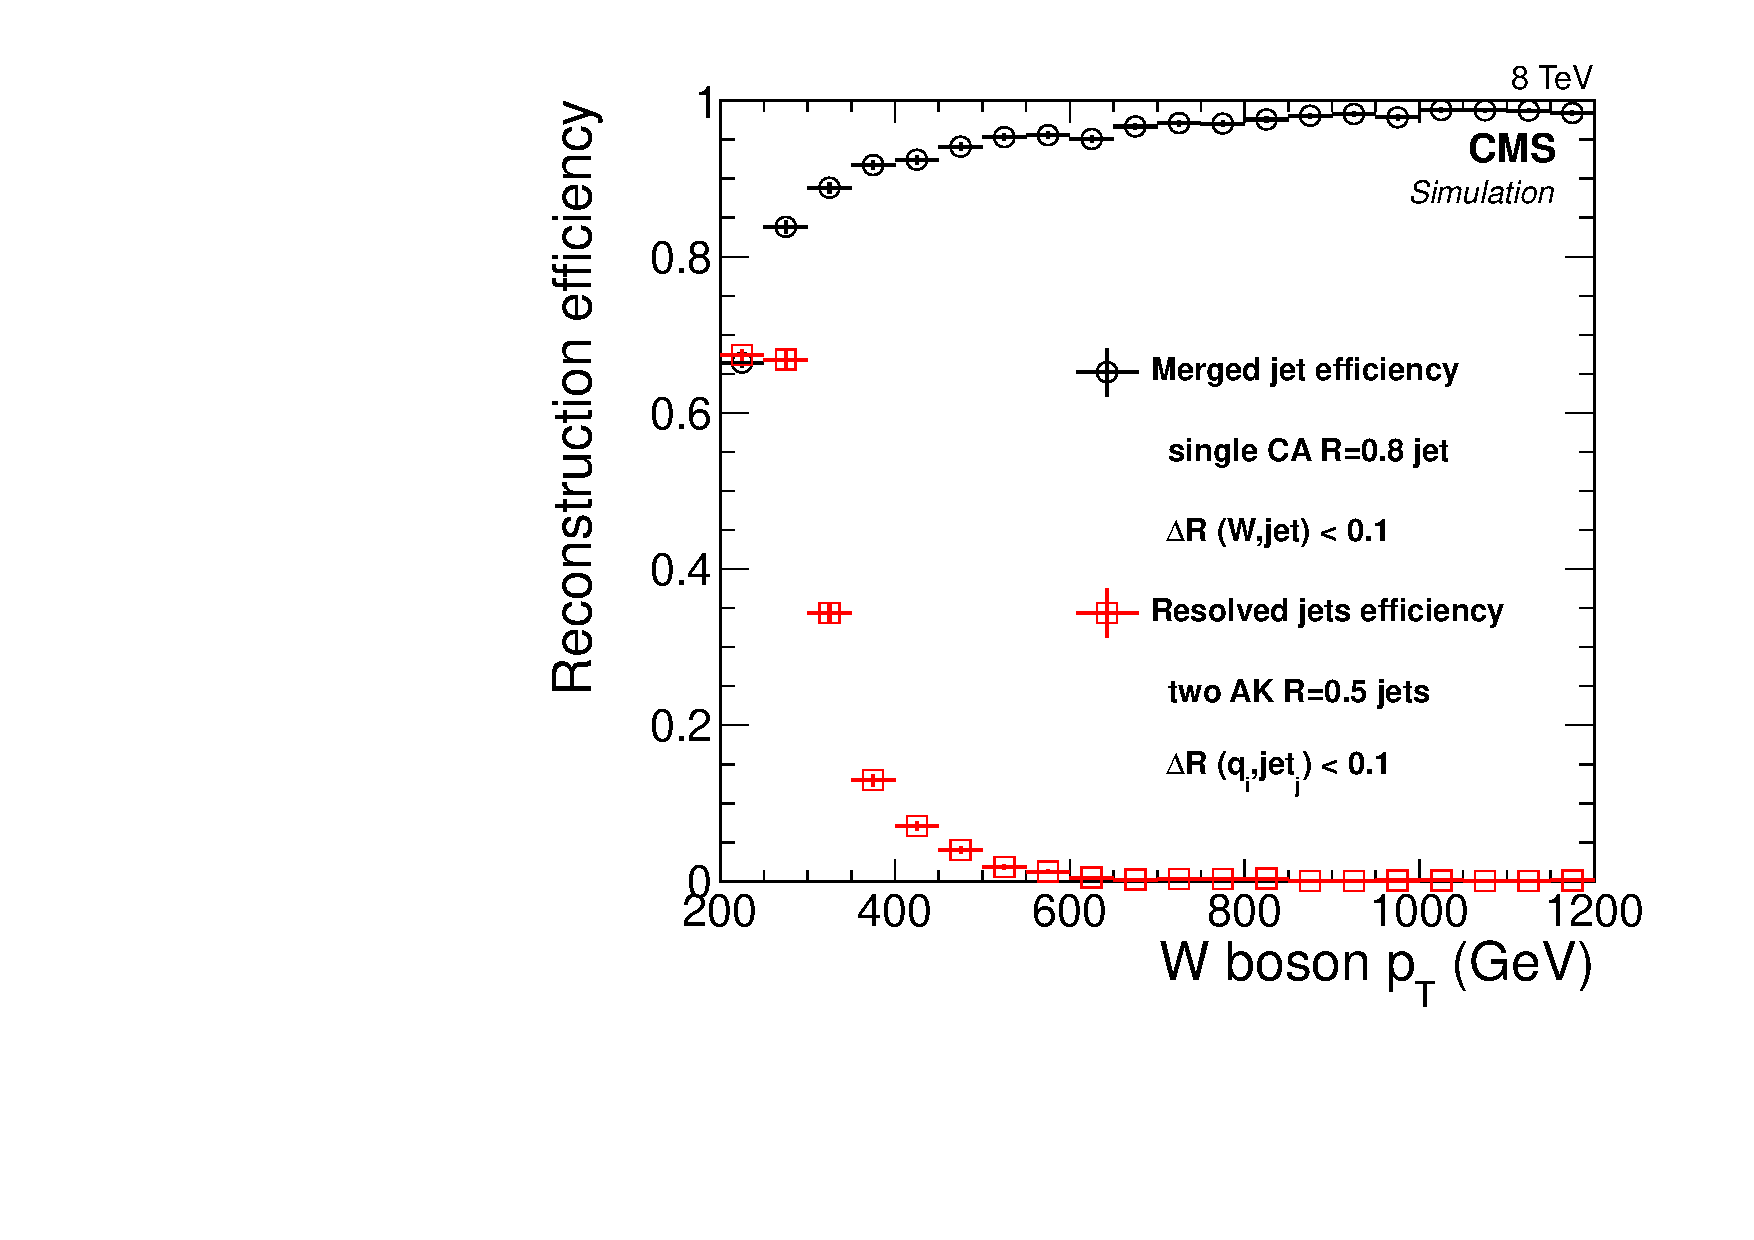
\includegraphics[width=0.5\textwidth]{\chsix/ca8effVsPt.pdf}
 \end{center}
 \caption{Efficiency to reconstruct a CA8 jet within $\Delta R <$ 0.1 of a generated W boson, and the efficiency to reconstruct two AK5 jets within $\Delta R <$ 0.1 of the generated quarks W bosons, as a function of the \pt of the W boson~\cite{Khachatryan:2014vla}.}
 \label{fig:ca8effVsPt}
\end{figure}

%%%%%%%% 
\subsection{Jet reconstruction and calibration}\label{subsec:jetsreco}
%%%%%%%%

%%%%%%%% 
\subsection{Identification of b jets}\label{subsec:bjets}
%%%%%%%%
